\section{Creazione DB}
In questa sezione verrà descritta la progettazione e la creazione del database. Il database è stato progettato per soddisfare i requisiti del sistema di monitoraggio e controllo di missioni spaziali e in modo da garantire la corretta memorizzazione e gestione dei dati relativi a missioni, membri dell'equipaggio, sensori, robot, anomalie, rilevazioni e report.

\subsection{Progettazione Concettuale}

La progettazione concettuale è la fase iniziale del processo di progettazione di un database, in cui si definiscono i requisiti del sistema e si identificano le entità coinvolte, le relazioni tra di esse e gli attributi che le caratterizzano. Questa fase è indipendente dal modello logico e si concentra sulla rappresentazione dei dati in modo astratto, senza considerare i dettagli implementativi. \\
La progettazione concettuale è stata realizzata attraverso la modellazione del sistema tramite il modello Entità/Relazione (E/R). Questo modello consente di rappresentare in modo chiaro e intuitivo le entità coinvolte, le relazioni tra di esse e gli attributi che le caratterizzano.

\subsubsection{Modello E/R portante}

Come prima fase della progettazione concettuale, è stato realizzato uno schema E/R portante. Lo schema portante rappresenta il nucleo centrale del modello Entità-Relazione (E/R) per il sistema in esame. Esso evidenzia le principali entità coinvolte: \textbf{RISORSA}, \textbf{MISSIONE} e \textbf{MEMBRO EQUIPAGGIO}, connesse tra loro tramite relazioni chiave.

\begin{itemize}
    \item La \textbf{RISORSA} rappresenta gli strumenti o gli elementi utilizzati nelle missioni.
    \item La \textbf{MISSIONE} è il fulcro operativo, dove vengono assegnate risorse e membri dell'equipaggio.
    \item Il \textbf{MEMBRO EQUIPAGGIO} indica le persone coinvolte nelle missioni, con specifici ruoli e compiti.
\end{itemize}

Le relazioni descrivono i collegamenti logici tra queste entità, evidenziando l'assegnazione e l'utilizzo di risorse e personale in contesto missione. Questo schema costituisce la base per la progettazione logica e fisica del sistema.

\begin{figure}[h!]
    \centering
    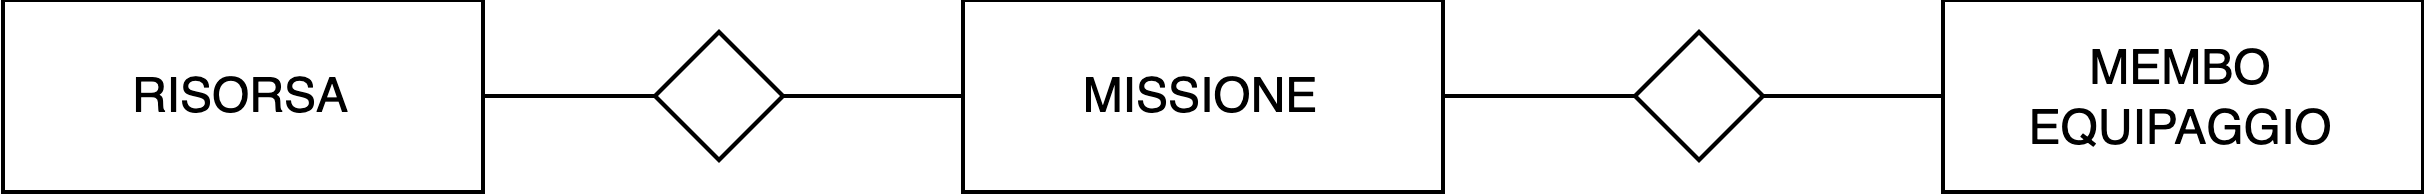
\includegraphics[width=1\textwidth]{Media/schema_portante.png}
    \caption{Schema portante del modello E/R}
    \label{fig:schema_portante}
\end{figure}


\subsubsection{Modello E/R completo}

A partire dallo schema portante descritto in precedenza, è stato realizzato uno schema E/R completo che include tutte le entità e le relazioni coinvolte nel sistema. Lo schema completo rappresenta in modo esaustivo tutte le entità, le relazioni e gli attributi che caratterizzano il sistema di monitoraggio e controllo di missioni spaziali.

\begin{figure}[h!]
    \centering
    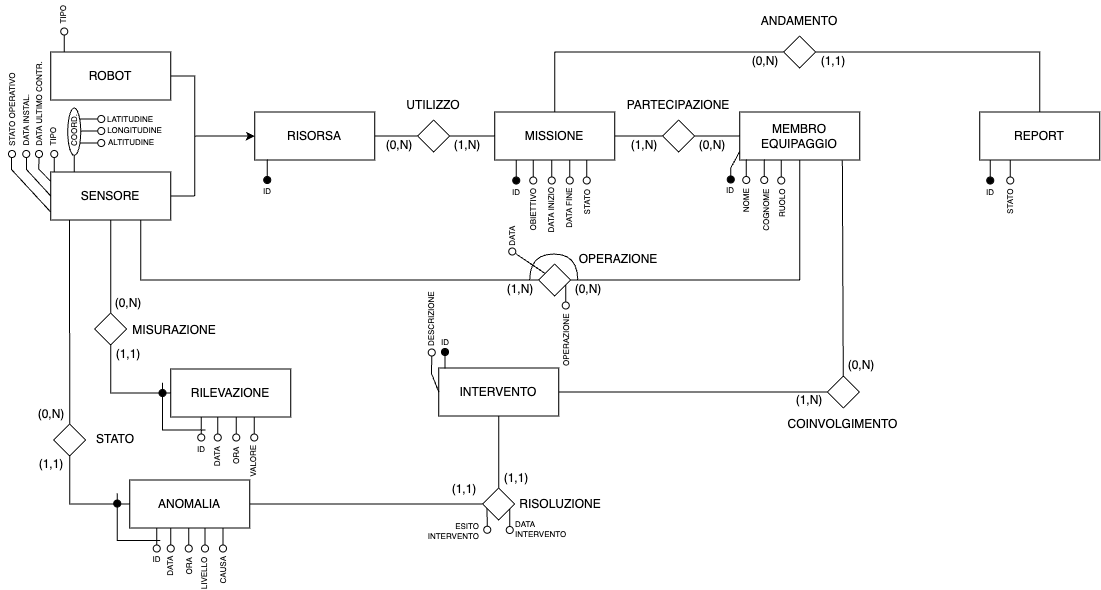
\includegraphics[width=0.8\textwidth]{Media/ER_Completo.png}
    \caption{Modello E/R completo}
    \label{fig:schema_portante}
\end{figure}

\paragraph{Specifiche di Progettazione}

TODO

\subsection{Progettazione Logica}

La progettazione logica si articola in due fasi:

\begin{enumerate}
    \item \textbf{Trasformazione}: in questa fase, vengono rimossi tutti i costrutti del modello Entità/Relazione (E/R) che non sono direttamente traducibili nel modello logico, come gli attributi composti e gli attributi multi-valore. Gli attributi multi-valore vengono associati direttamente all’entità di partenza, mentre gli attributi composti vengono scomposti nei loro componenti e, se necessario, trasferiti a una nuova entità collegata all’entità originale.
    \item \textbf{Traduzione}: lo schema risultante dalla trasformazione viene convertito nel modello logico attraverso un insieme di regole predeterminate, che possono essere implementate anche tramite strumenti automatizzati. Questa fase non considera direttamente la semantica dei dati, ma si concentra sulla loro struttura.
\end{enumerate}

\subsubsection{Trasformazione}

Durante la fase di trasformazione, vengono eliminati tutti gli attributi che non sono direttamente traducibili nel modello logico. Di seguito vengono descritti i casi specifici presenti nello schema:

\begin{itemize}
    \item \textbf{Attributi multi-valore}: non sono presenti in questo caso, quindi non si rende necessaria alcuna operazione di trasformazione relativa a questa tipologia di attributi.
    \item \textbf{Attributi composti}: l'unico attributo composto identificato è \textbf{Coordinate}, associato all'entità \textit{SENSORE}. Per conformarsi ai requisiti del modello logico, questo attributo è stato scomposto nei suoi componenti: \textbf{Latitudine}, \textbf{Longitudine} e \textbf{Altitudine}. Tali componenti sono stati direttamente associati all’entità di partenza senza creare una nuova entità.
\end{itemize}

Di seguito è riportato lo schema trasformato per l'entità \textit{SENSORE}:\\

\begin{figure}[h!]
    \centering
    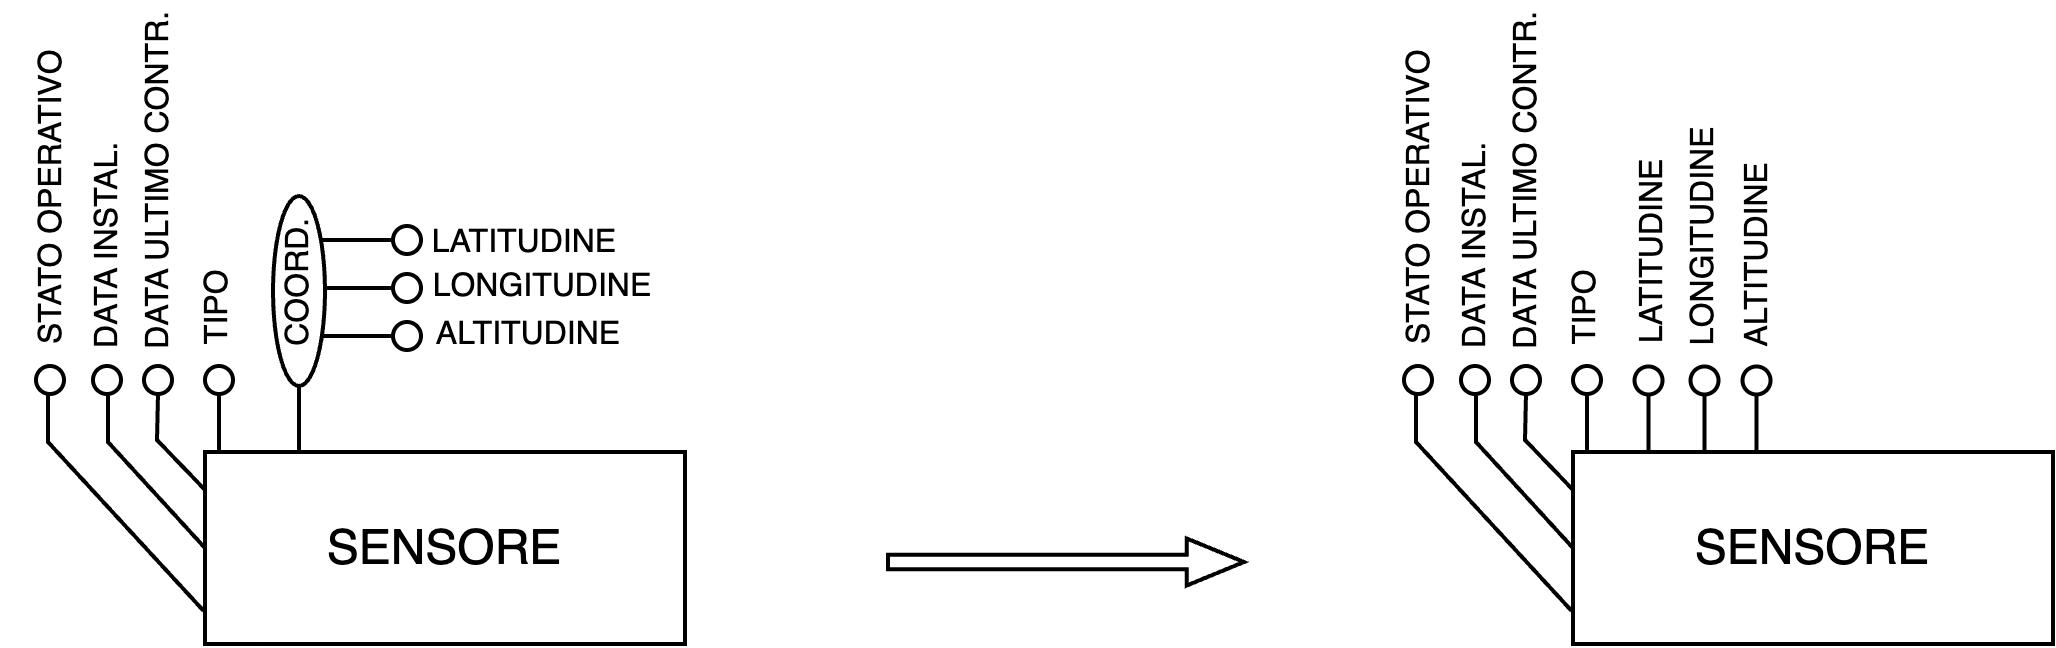
\includegraphics[width=0.8\textwidth]{Media/Trasformazione_Sensore.png}
    \caption{Entità \textit{SENSORE} trasformata}
    \label{fig:schema_portante}
\end{figure}

\subsubsection{Traduzione}

TODO: DESCRIZIONE FASE TRADUZIONE

\paragraph{Traduzione Entità}

Ogni entità del modello E/R diventa una relazione/tabella.
\begin{itemize}
    \item \textbf{Nome della tabella}: corrisponde al nome dell’entità.
    \item \textbf{Campi della tabella}: corrispondono agli attributi dell’entità.
\end{itemize}

Risultato della Traduzione delle Entità:
\begin{lstlisting}
MISSIONI(ID, Obiettivo, Data_Inizio, Data_Fine, Stato);
MEMBI(ID, Nome, Cognome, Ruolo);
REPORT(ID, Stato);
INTERVENTI(ID, Descrizione);
ANOMALIE(ID, Data, Ora, Livello, Causa);
RILEVAZIONI(ID, Data, Ora, Valore);
ROBOT(ID, Tipo);
SENSORI(ID, Data_Installazione, Data_Ultimo_Controllo, Tipo, Stato_Operativo, Latitudine, Longitudine, Altitudine)
\end{lstlisting}

\paragraph{Traduzione Relazioni}
\begin{enumerate}
    \item Relazioni \textbf{N a N}
    \begin{itemize}
        \item Ogni associazione N a N diventa una tabella con:
        \begin{itemize}
            \item \textbf{Nome}: corrisponde al nome dell’associazione, al plurale.
            \item \textbf{Campi}: includono gli identificatori delle due entità che collega, più eventuali attributi dell’associazione.
            \item \textbf{Chiave primaria}: composta dalla coppia dei due identificatori.
            \item \textbf{Vincoli di integrità referenziale}: garantiscono la consistenza con le entità collegate.
        \end{itemize}
    \end{itemize}
    \begin{lstlisting}
    UTILIZZO_SENSORI (Sensore: Sensori, Missione: Missioni);
    UTILIZZO_ROBOT (Robot: Robot, Missione: Missioni);
    PARTECIPAZIONI (Missione: Missioni, Membro_Equipaggio: Membri_Equipaggio);
    OPERAZIONI (Membro_Equipaggio: Membri_Equipaggio, Sensore: Sensori, Operazione, Data);
    COINVOLGIMENTI (Membro_Equipaggio: Membri_Equipaggio, Intervento: Interventi)
    \end{lstlisting}

    \item Relazioni \textbf{1 a N}
    \begin{itemize}
        \item Gli \textbf{attributi dell’entità lato 1} e gli \textbf{attributi della relazione} vengono aggiunti come campi all’entità lato N.
        \item \textbf{Chiave primaria}: rimane quella dell’entità lato N.
        \item Questa scelta consente di ridurre il numero di tabelle, evitando join complessi a 3 tabelle.
    \end{itemize}
    \begin{lstlisting}
    REPORT (ID, Stato, Data, Missione: Missioni);
    RILEVAZIONI (ID, Data, Ora, Valore, Sensore: Sensori);
    ANOMALIE (ID, Data, Ora, Livello, Causa, Sensore: Sensori);
    \end{lstlisting}

    \item Relazioni \textbf{1 a 1}
    \begin{itemize}
        \item Ogni associazione 1 a 1 diventa una tabella con:
        \begin{itemize}
            \item \textbf{Campi}: includono gli identificatori delle entità che collega, più eventuali attributi.
            \item \textbf{Chiave primaria}: si sceglie l’identificatore dell’entità con cardinalità minima e partecipazione obbligatoria, per evitare valori NULL.
        \end{itemize}
    \end{itemize}
    \begin{lstlisting}
    RISOLUZIONI (Intervento: Interventi, Anomalia: Anomalie, Esito_Intervento, Data_Intervento)
    \end{lstlisting}
\end{enumerate}

\subsubsection{Modello E/R avanzato}

Le gerarchie di generalizzazione/specializzazione non possono essere direttamente rappresentate nel modello logico relazionale, poiché quest'ultimo non prevede un costrutto equivalente. Per superare questa limitazione, il modello E/R è stato esteso con l'introduzione del costrutto di \textbf{generalizzazione/specializzazione}. \\

Il costrutto di generalizzazione può essere trasformato in schemi traducibili nel modello logico seguendo tre modalità principali.\\

Per questo progetto è stata adottata la modalità di \textbf{accorpamento della superclasse nelle sottoclassi}:
\begin{itemize}
    \item \textbf{Eliminazione dell’entità padre}: l'entità padre (superclasse) viene eliminata dallo schema.
    \item \textbf{Eredità degli attributi e delle relazioni}: grazie alla proprietà dell’eredità, gli attributi, l’identificatore e le relazioni a cui partecipava l’entità padre vengono trasferiti integralmente alle entità figlie (sottoclassi).
\end{itemize}

Di seguito è riportato il risultato dell'accorpamento relativo alla superclasse \textit{RISORSA} e alle sottoclassi \textit{ROBOT} e \textit{SENSORE}

\begin{figure}[h!]
    \centering
    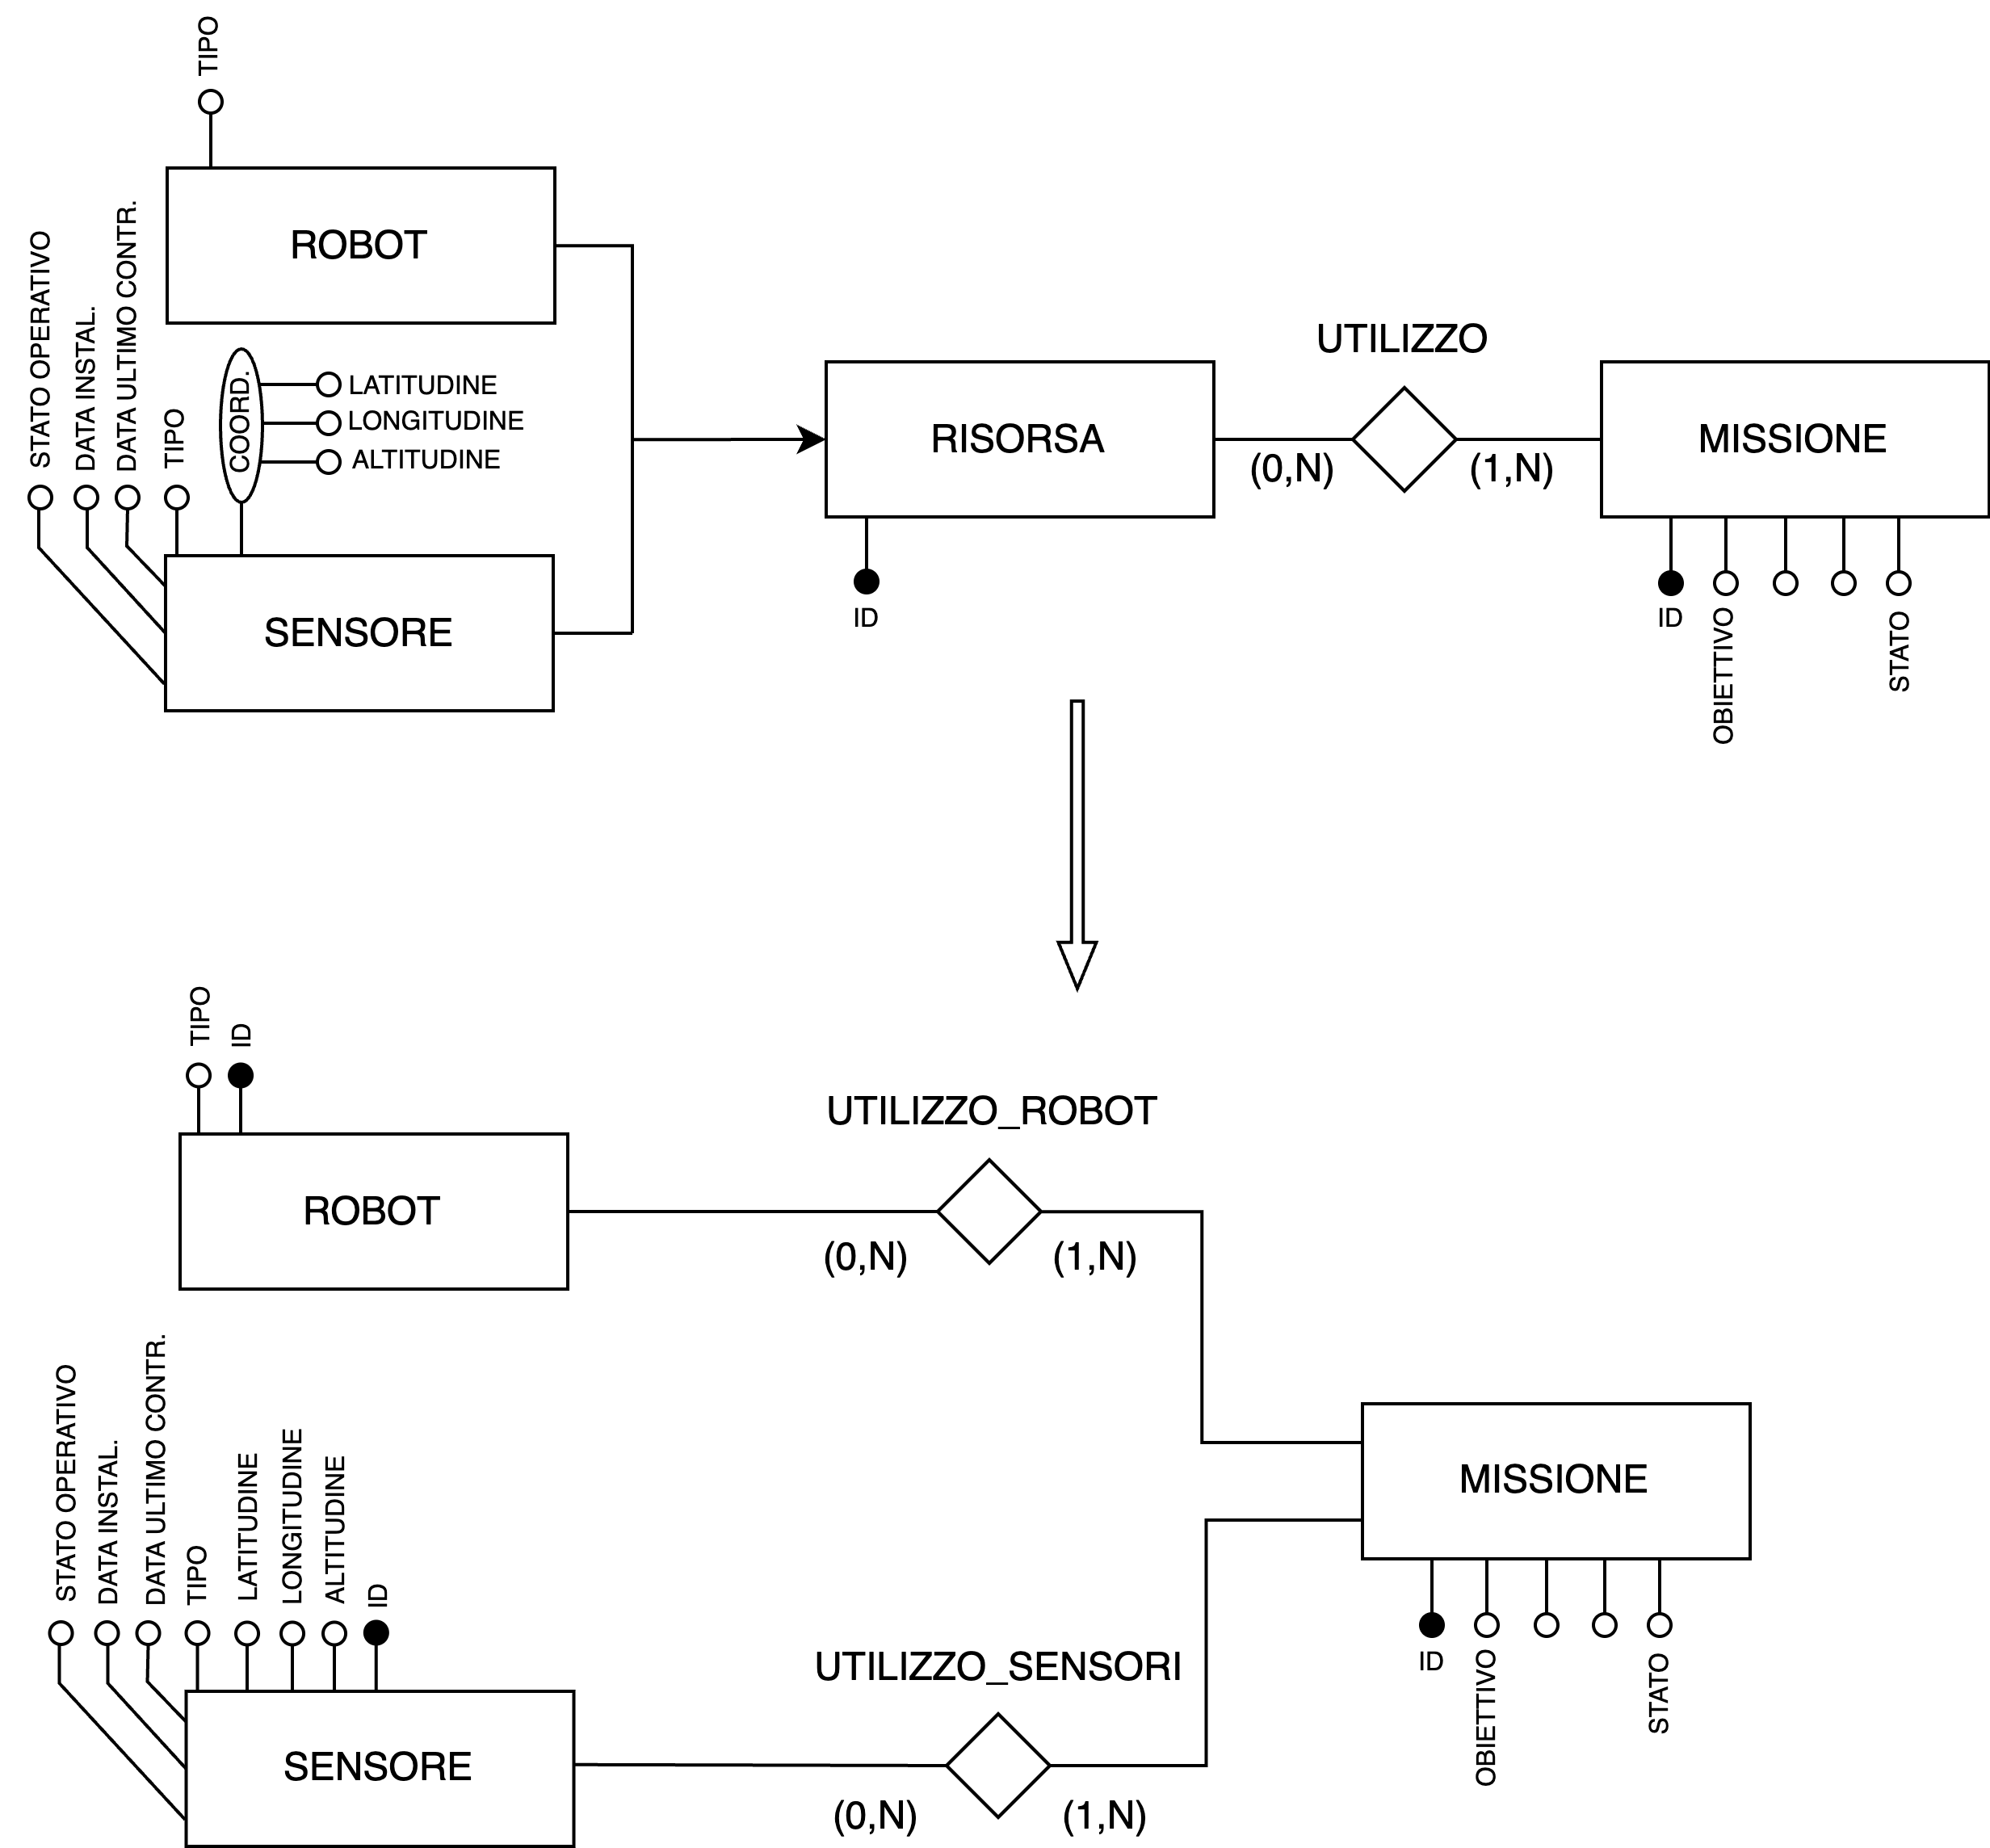
\includegraphics[width=0.8\textwidth]{Media/Generalizzazione_Specializzazione.png}
    \caption{accorpamento di \textit{RISORSA} in \textit{ROBOT} e \textit{SENSORE}}
    \label{fig:schema_portante}
\end{figure}

\subsection{Progettazione Fisica}

I tipi di dato utilizzati per la realizzazione di questo progetto sono:

\begin{itemize}
    \item \textbf{DATE}: Utilizzato per tutte le date presenti.
    \item \textbf{INTEGER}: per tutti gli ID che quindi sono formati esclusivamente da numeri e non da lettere;
    \item \textbf{VARCHAR2(N)}: per tutti gli attributi di tipo testuali, come per esempio nome, cognome, descrizione, ecc..
\end{itemize}

\subsubsection{Tabelle}

\begin{lstlisting}
-- Tabella MISSIONI
CREATE TABLE MISSIONI (
    ID INT,
    Obiettivo VARCHAR2(255) NOT NULL,
    Data_Inizio DATE NOT NULL, --NOT NULL o no ?
    Data_Fine DATE,
    Stato VARCHAR2(50) NOT NULL
);

-- Tabella MEMBRI
CREATE TABLE MEMBRI (
    ID INT,
    Nome VARCHAR2(100) NOT NULL,
    Cognome VARCHAR2(100) NOT NULL,
    Ruolo VARCHAR2(100) NOT NULL
);

-- Tabella SENSORI
CREATE TABLE SENSORI (
    ID INT,
    Data_Installazione DATE NOT NULL,
    Data_Ultimo_Controllo DATE,
    Tipo VARCHAR2(100) NOT NULL,
    Latitudine FLOAT NOT NULL,
    Longitudine FLOAT NOT NULL,
    Altitudine FLOAT NOT NULL
);

-- Tabella ROBOT
CREATE TABLE ROBOT (
    ID INT,
    Tipo VARCHAR2(100) NOT NULL
);

-- Tabella ANOMALIE
CREATE TABLE ANOMALIE (
    ID INT,
    Data DATE NOT NULL,
    Ora TIMESTAMP NOT NULL,
    Livello VARCHAR2(50) NOT NULL,
    Causa VARCHAR2(255) NOT NULL,
    Sensori INT
);

-- Tabella INTERVENTI
CREATE TABLE INTERVENTI (
    ID INT,
    Descrizione VARCHAR2(255) NOT NULL
);

-- Tabella RISOLUZIONI
CREATE TABLE RISOLUZIONI (
    Anomalie INT,
    Interventi INT,
    Esito_Intervento VARCHAR2(255),
    Data_Intervento DATE
);

-- Tabella RILEVAZIONI
CREATE TABLE RILEVAZIONI (
    ID INT,
    Data DATE NOT NULL,
    Ora TIMESTAMP NOT NULL,
    Valore FLOAT NOT NULL,
    Sensori INT
);

-- Tabella REPORT
CREATE TABLE REPORT (
    ID INT,
    Stato VARCHAR2(50) NOT NULL,
    Missioni INT
);

-- Tabella UTILIZZO_ROBOT
CREATE TABLE UTILIZZO_ROBOT (
    Robot INT,
    Missioni INT
);

-- Tabella UTILIZZO_SENSORI
CREATE TABLE UTILIZZO_SENSORI (
    Sensori INT,
    Missioni INT
);

-- Tabella COINVOLGIMENTI
CREATE TABLE COINVOLGIMENTI (
    Membri INT,
    Interventi INT
);

-- Tabella OPERAZIONI
CREATE TABLE OPERAZIONI (
    Membri INT,
    Sensori INT,
    Stato_Operativo VARCHAR2(50) NOT NULL,
    Operazione VARCHAR2(255)
);

-- Tabella PARTECIPAZIONI
CREATE TABLE PARTECIPAZIONI (
    Missione INT,
    Membri INT
);

-- Tabella SENSORI_MISSIONI
CREATE TABLE SENSORI_MISSIONI (
    Sensore_ID INT,
    Missione_ID INT,
    PRIMARY KEY (Sensore_ID, Missione_ID),
    FOREIGN KEY (Sensore_ID) REFERENCES SENSORI(ID),
    FOREIGN KEY (Missione_ID) REFERENCES MISSIONI(ID)
);

-- Tabella MEMBRI_MISSIONI
CREATE TABLE MEMBRI_MISSIONI (
    Membro_ID INT,
    Missione_ID INT,
    PRIMARY KEY (Membro_ID, Missione_ID),
    FOREIGN KEY (Membro_ID) REFERENCES MEMBRI(ID),
    FOREIGN KEY (Missione_ID) REFERENCES MISSIONI(ID)
);
\end{lstlisting}

\subsubsection{Chiavi primarie}

\begin{lstlisting}
ALTER TABLE MISSIONI ADD CONSTRAINT PK_MISSIONI PRIMARY KEY (ID);
ALTER TABLE MEMBRI ADD CONSTRAINT PK_MEMBRI PRIMARY KEY (ID);
ALTER TABLE SENSORI ADD CONSTRAINT PK_SENSORI PRIMARY KEY (ID);
ALTER TABLE ROBOT ADD CONSTRAINT PK_ROBOT PRIMARY KEY (ID);
ALTER TABLE ANOMALIE ADD CONSTRAINT PK_ANOMALIE PRIMARY KEY (ID);
ALTER TABLE INTERVENTI ADD CONSTRAINT PK_INTERVENTI PRIMARY KEY (ID);
ALTER TABLE RILEVAZIONI ADD CONSTRAINT PK_RILEVAZIONI PRIMARY KEY (ID);
ALTER TABLE REPORT ADD CONSTRAINT PK_REPORT PRIMARY KEY (ID);
ALTER TABLE RISOLUZIONI ADD CONSTRAINT PK_RISOLUZIONI PRIMARY KEY (Anomalie, Interventi);
ALTER TABLE UTILIZZO_ROBOT ADD CONSTRAINT PK_UTILIZZO_ROBOT PRIMARY KEY (Robot, Missioni);
ALTER TABLE UTILIZZO_SENSORI ADD CONSTRAINT PK_UTILIZZO_SENSORI PRIMARY KEY (Sensori, Missioni);
ALTER TABLE COINVOLGIMENTI ADD CONSTRAINT PK_COINVOLGIMENTI PRIMARY KEY (Membri, Interventi);
ALTER TABLE OPERAZIONI ADD CONSTRAINT PK_OPERAZIONI PRIMARY KEY (Membri, Sensori);
ALTER TABLE PARTECIPAZIONI ADD CONSTRAINT PK_PARTECIPAZIONI PRIMARY KEY (Missione, Membri);
\end{lstlisting}

\subsubsection{Chiavi esterne}

\begin{lstlisting}
ALTER TABLE ANOMALIE ADD CONSTRAINT FK_ANOMALIE_SENSORI FOREIGN KEY (Sensori) REFERENCES SENSORI(ID);
ALTER TABLE RISOLUZIONI ADD CONSTRAINT FK_RISOLUZIONI_ANOMALIE FOREIGN KEY (Anomalie) REFERENCES ANOMALIE(ID);
ALTER TABLE RISOLUZIONI ADD CONSTRAINT FK_RISOLUZIONI_INTERVENTI FOREIGN KEY (Interventi) REFERENCES INTERVENTI(ID);
ALTER TABLE RILEVAZIONI ADD CONSTRAINT FK_RILEVAZIONI_SENSORI FOREIGN KEY (Sensori) REFERENCES SENSORI(ID);
ALTER TABLE REPORT ADD CONSTRAINT FK_REPORT_MISSIONI FOREIGN KEY (Missioni) REFERENCES MISSIONI(ID);
ALTER TABLE UTILIZZO_ROBOT ADD CONSTRAINT FK_UTILIZZO_ROBOT_ROBOT FOREIGN KEY (Robot) REFERENCES ROBOT(ID);
ALTER TABLE UTILIZZO_ROBOT ADD CONSTRAINT FK_UTILIZZO_ROBOT_MISSIONI FOREIGN KEY (Missioni) REFERENCES MISSIONI(ID);
ALTER TABLE UTILIZZO_SENSORI ADD CONSTRAINT FK_UTILIZZO_SENSORI_SENSORI FOREIGN KEY (Sensori) REFERENCES SENSORI(ID);
ALTER TABLE UTILIZZO_SENSORI ADD CONSTRAINT FK_UTILIZZO_SENSORI_MISSIONI FOREIGN KEY (Missioni) REFERENCES MISSIONI(ID);
ALTER TABLE COINVOLGIMENTI ADD CONSTRAINT FK_COINVOLGIMENTI_MEMBRI FOREIGN KEY (Membri) REFERENCES MEMBRI(ID);
ALTER TABLE COINVOLGIMENTI ADD CONSTRAINT FK_COINVOLGIMENTI_INTERVENTI FOREIGN KEY (Interventi) REFERENCES INTERVENTI(ID);
ALTER TABLE OPERAZIONI ADD CONSTRAINT FK_OPERAZIONI_MEMBRI FOREIGN KEY (Membri) REFERENCES MEMBRI(ID);

ALTER TABLE OPERAZIONI ADD CONSTRAINT FK_OPERAZIONI_SENSORI FOREIGN KEY (Sensori) REFERENCES SENSORI(ID);

ALTER TABLE PARTECIPAZIONI ADD CONSTRAINT FK_PARTECIPAZIONI_MISSIONE FOREIGN KEY (Missione) REFERENCES MISSIONI(ID);

ALTER TABLE PARTECIPAZIONI ADD CONSTRAINT FK_PARTECIPAZIONI_MEMBRI FOREIGN KEY (Membri) REFERENCES MEMBRI(ID);
\end{lstlisting}

\subsubsection{Vincoli di check}

\begin{lstlisting}
    ALTER TABLE SENSORI ADD CONSTRAINT CK_SENSORI_TIPO CHECK (Tipo IN ('Temperatura', 'Pressione', 'Gas', 'Radiazioni', 'Geologia'));
    
    ALTER TABLE OPERAZIONI ADD CONSTRAINT CK_OPERAZIONI_STATO CHECK (Stato_Operativo IN ('Attivo', 'Standby', 'Manutenzione', 'Malfunzionante'));
    
    ALTER TABLE ANOMALIE ADD CONSTRAINT CK_ANOMALIE_LIVELLO CHECK (Livello IN ('Bassa', 'Media', 'Alta', 'Critica'));
    
    ALTER TABLE MISSIONI ADD CONSTRAINT CK_MISSIONI_STATO CHECK (Stato IN ('Pianificata', 'In corso', 'Completata', 'Annullata'));
\end{lstlisting}

